\begin{figure}[h!]
	\centering{
		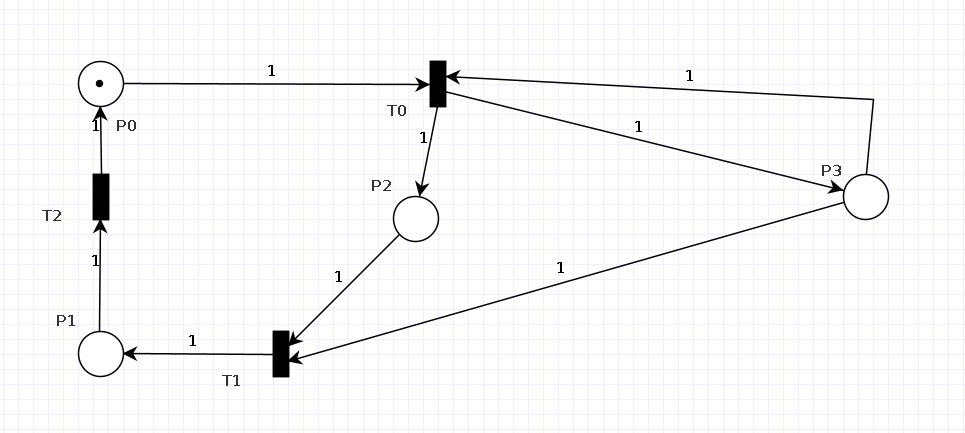
\includegraphics[width=0.67\textwidth]{img/21.png}
	}
	\caption{Sieć z podanego przykładu}
	\label{zad2:graph1}
\end{figure}

\begin{figure}[h!]
	\centering{
		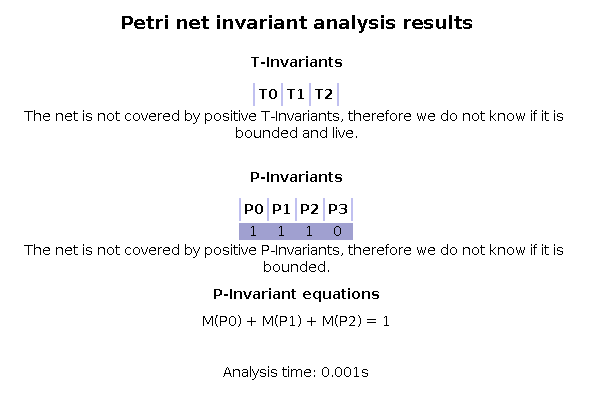
\includegraphics[width=0.67\textwidth]{img/23.png}
	}
	\caption{Niezmienniki sieci z podanego przykładu}
	\label{zad2:graph1}
\end{figure}
\begin{figure}[h!]
	\centering{
		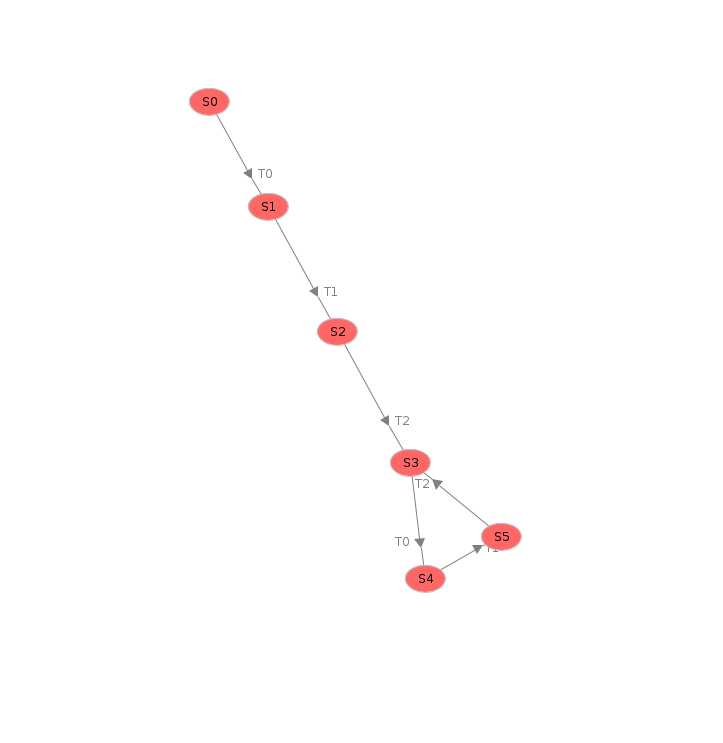
\includegraphics[width=0.67\textwidth]{img/2_3.png}
	}
	\caption{Graf osiągalności}
	\label{zad2:graph1}
\end{figure}
\newpage
\subsection{Graf osiągalności}
W miejscu $P_3$ może wystąpić dowolnie duża liczba, więc graf osiągalności jest nieskończony.
\subsection{Analiza niezminników przejść}
Sieć nie jest odwracalna, ponieważ tranzycja $T_2$ będzie za każdym razem na-
mnażać znaczników w miejscu $P_1$. Z tego powodu po jej wywołaniu nie da się już powrócić
do znakowania początkowego.